%%%%%%%%%%%%%%%%%%%%%%%%%%%%%%%%%%%%%%%%%%%%%%%%%%%%%%%%%%%%%%%%%%%%%%%%%%%%%%%%
%%%%%%%%%%%%%%%%%%%%%%%%%%%%%%%%%%%%%%%%%%%%%%%%%%%%%%%%%%%%%%%%%%%%%%%%%%%%%%%%
\section{\textcolor{red}{Contando e medindo a frase musical}}
\index{Musicalidade!Frase musical}
\cite[pp. 148,150]{medteoria}

\cite[pp. 336]{medteoria}

o cumprimento de frase mais comum é
de 4 compassos \cite[pp. 624]{latham2008diccionario} \cite[pp. 335]{medteoria} \cite[pp. 34]{bennett1993elementos},
tabem é usado cumprimentos de 8 compassos \cite[pp. 335]{medteoria} \cite[pp. 34]{bennett1993elementos}
e 2 compassos \cite[pp. 34]{bennett1993elementos}.
São menos comuns frases de 3,5, ou 7 compassos \cite[pp. 34]{bennett1993elementos}.

Ver Figura \ref{fig:contagemtemposfrase}.
\begin{figure}
    \centering
    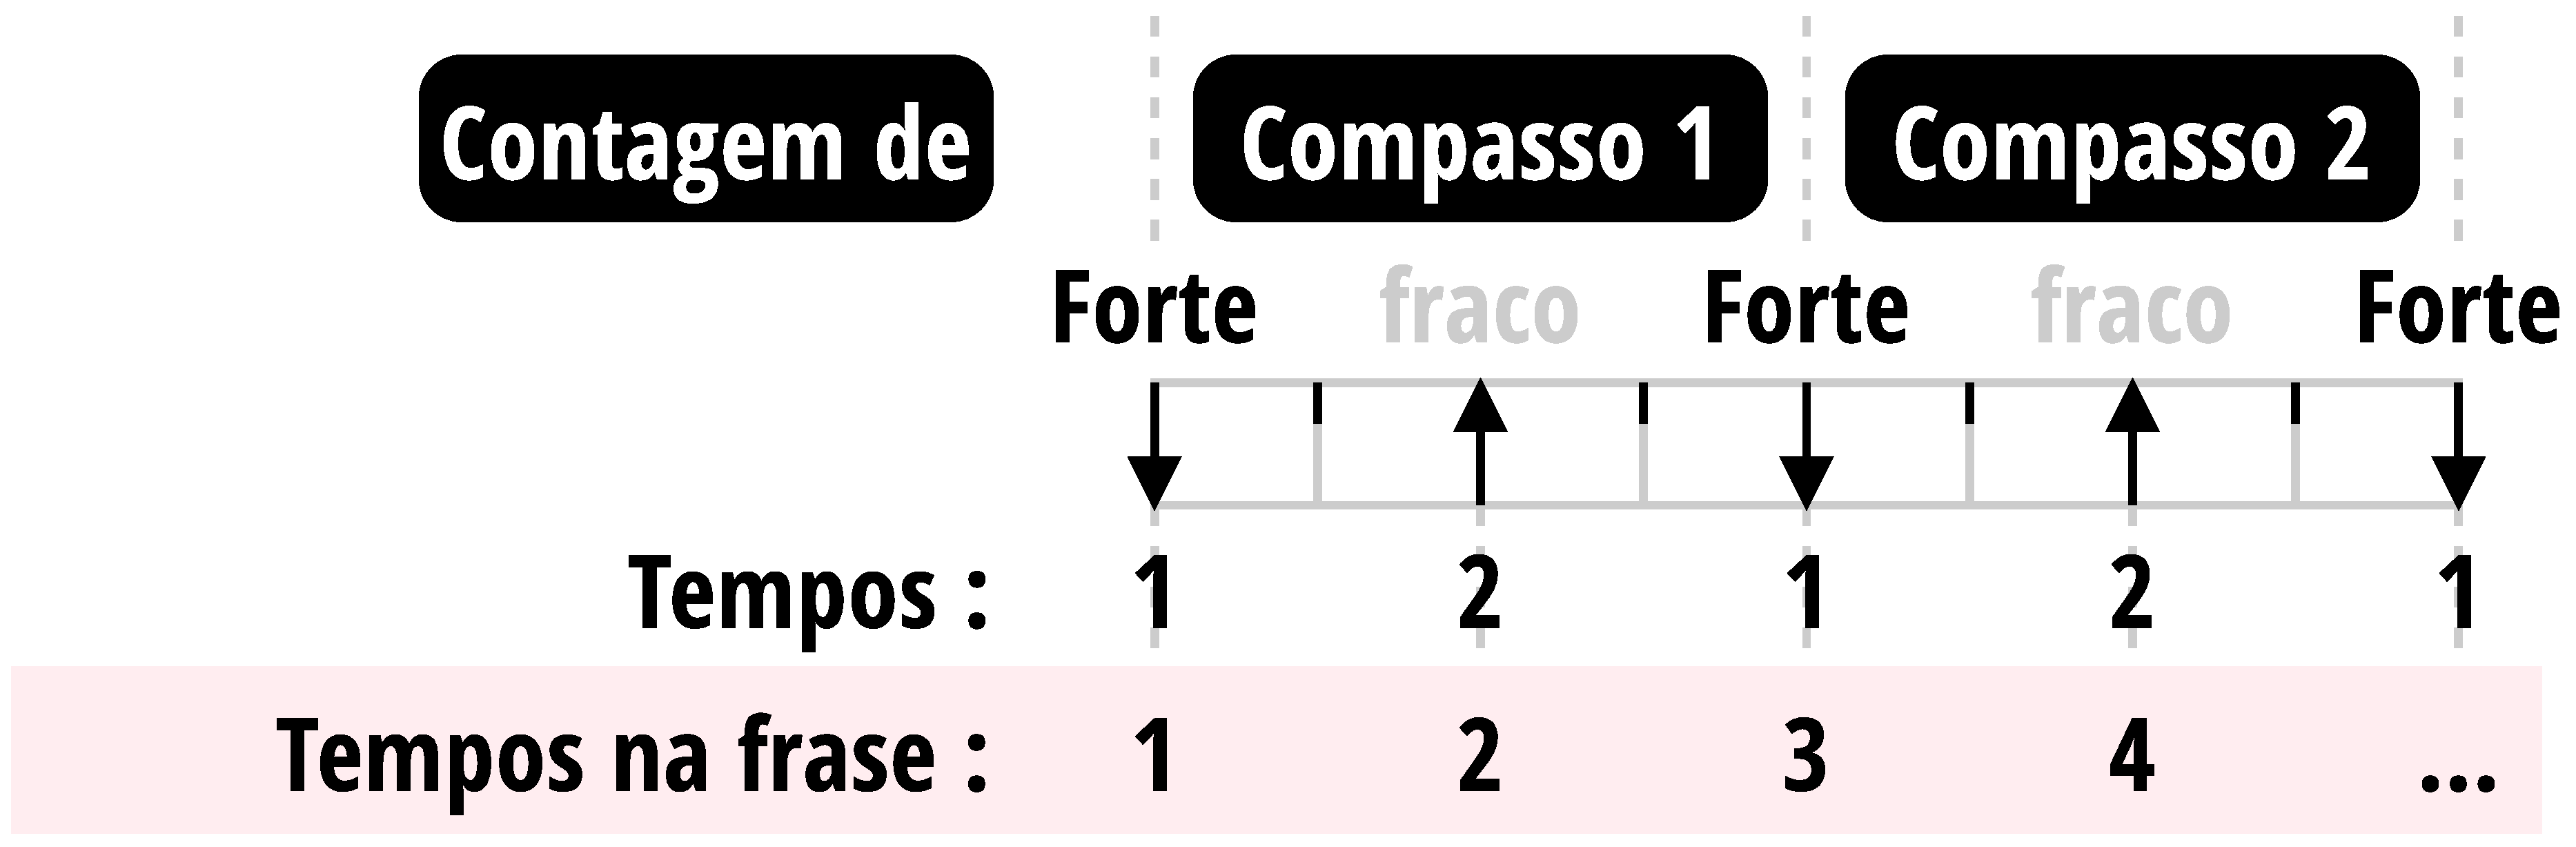
\includegraphics[width=\textwidth]{chapters/cap-musicalidade/contagemtemposfrase.eps}
    \caption{Contando a frase musical.}
    \label{fig:contagemtemposfrase}
\end{figure}

